\documentclass{standalone}
% preamble: usepackage, etc.
\begin{document}
	
\chapter{系统测试与分析}
\section{系统测试}
本文的测试分为两个部分,第一部分是单例测试,在单例测试中会从
最原始的文本输入开始讲解,系统前后端是如何通信的以及前后端
协议的数据格式,然后详细介绍系统后端是如何进行问题求解的,
各个模块是否完成了对应的功能以及各个逻辑层之间是否完成连通,
在此基础上验证系统的整体流程是否流通,保证最后的结果输出
和类人解答过程的生成;第二部分是批量测试,批量测试是随机选定
各个不同知识模块200题,共1000题形成的测试集,其中涉及到函数、
数列、向量、解析几何、平面几何等知识模块,系统在测试集上进行
测试,通过统计测试的结果,来反馈系统中存在那些不足,对系统的
缺陷进行深入分析,归类错误类型,从而增强系统的稳定性、可靠性
和兼容性。另外,批量测试还能够去检验概念知识图谱和实例化定理库
的完备性。
\subsection{单例测试}
单例测试是从一道题目的原始描述文本开始进行输入,依次进行不同
模块测试:题目文本的自然语言理解,这里是测试自然语言理解中的
命名实体和关系抽取是否正确;题目Json数据生成知识图谱中的子图,
这里是测试生成的题目子图知识信息是否完整;预处理模块的知识
扩展,测试预处理模块对隐含知识的扩展是否正确;图同构的推理引擎,
这里主要是测试推理引擎的三个逻辑层的具体实现模块是否正常运行,
三元组匹配模块、变量置换模块、知识更新模块能否连通成功;
类人解答过程,测试系统是否正确停机并且输出类人解答过程。

本次单例测试选取的题目是全国卷三文科的第17题,具体题目描述
为”设等比数列${a_n}$满足$a_1+a_2=4$,$a_3-a_1=8$,(1)则${a_n}$
的通项公式为;(2)记$S_n$为数列$b_n={log[3](a_n)}$的前n项和,
若$S_m+S_(m+1)=S_(m+3)$,求m“。首先对题目进行分析,第一问是
求解等比数列的通项公式,由通项公式的公式$a_n=a_1*q^(n-1)$可知
只需求出首项$a_1$和公比$q$即可,题干中已经有首项$a_1$,因此第一步
是通过实例化定理引入公比$q$,然后再将等比数列的项转换成首项和公比
表示,得到指包含首项$a_1$和公比q的两个方程,求解方程组便可求解出
$a_1$和$q$,进而求出通项公式;第二问的难点在于复合数列${log[3](a_n)}$,
依据第一问的通项公式可得到复合数列的通项公式,在利用前n项和$S_n$与
通项公式之间的关系,分别表示$S_m$、$S_(m+1)$、$S_(m+3)$,解方程即可得到
变量m的值。该题的解答过程如图5-1所示。
\begin{figure}[htbp]
	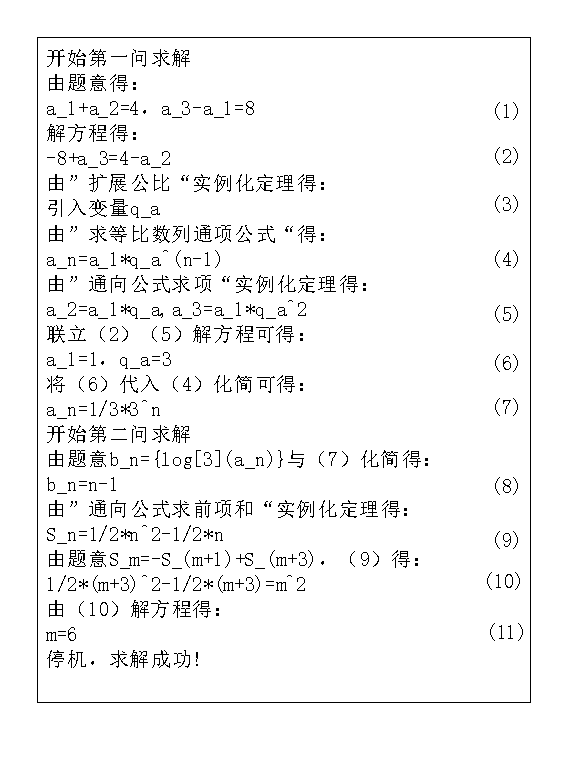
\includegraphics{类人解答过程文字.pdf}
	\caption{类人解答过程}
	\label{类人解答过程文字}
\end{figure}
前文详细介绍过实例化定理库是推理引擎重要的解题依据和驱动器,通过
刚刚对题目信息和求解目标的分析,首先确保实例化定理库中包含解题所
涉及到的知识定理或公式。本题具体使用到的实例化定理有”数列扩展公比“,
”已知首相和公比表示等比数列的项“,”求等比数列的通项公式“,”复合数列的
通向公式“,”已知通项公式求前n项和$S_n$“,”“。对应的实例化描述如表5-1所示。
\begin{table}[h]
	\caption{数列实例化定理} 
	\begin{tabular}{|c|c|l|} 
		\hline  
		定理标签 & 定理名称 & 描述 \\
		\hline  
		myBkFsvN & 数列扩展首项
		& \makecell[l]{已知数列$\{k_n\}$,\\则$\{k_n\}$的首项为$\#firstItem\#\{k_n\}$}\\  
		\hline  
		ieokuALX & 扩展公比
		& \makecell[l]{已知数列$\{k_n\}$,\\则$\{k_n\}$的公比为$\#qName\#\{k_n\}$}\\ 
		\hline  
		RwMkuGfC & 已知通向公式求前n项和
		& \makecell[l]{已知数列$\{k_n\}$的通项公式为$\{k_n\}=f(n)$,\\则$\{k_n\}$的前n项和为$\#sum\#\{k_n\}=f(n)$}\\ 
		\hline  
		jAkkuGfC & 求数列的前K项的和 
		& \makecell[l]{等差数列$\{k_n\}$的首项为$k_1$,\\$\{k_n\}$的公差为$t$,\\则$\#simp\#k_m=k_1+t*(m-1):k_1\&t\&k_m$}\\  
		\hline 
		 DegkuGfC & 求等比数列通项公式  
		& \makecell[l]{$\{k_n\}$为等比数列,\\$\{k_n\}$的首项为$k_1$,\\$\{k_n\}$的公比为$q$,\\则$\{k_n\}$的通项公式为$\#simp\#\{k_n\}=k_1*q^(n-1):\{k_n\}\&k_1\&q$}\\  
		\hline 
	\end{tabular}
	\label{tablea}
\end{table}


单例测试是在测试平台上进行的,测试的输入是由题目的输入和实例化定理的输入
两个部分组成。其中,题目的输入在测试平台上包含两部分,已知事实和求解目标在网页
端分开输入;实例化规则的输入也分成两部分输入,前提条件和结论。接下里,以3号实例
化规则为例,条件为”“,结论为”“,在网页端的传入如图5-2所示,选择的条件和结论的
三元组如图5-3所示。本题部分实例化定理对应的实例知识图谱分别如图
5-4(a)、5-4(b)、5-4(c)、5-4(d)所示,
\begin{figure}[htbp]
	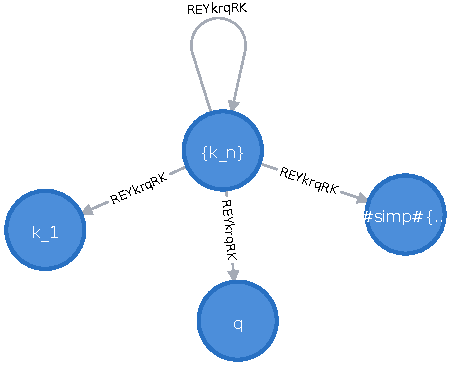
\includegraphics{前k项实例化.pdf}
	\caption{求前k项实例化图谱}
	\label{前k项实例化}
\end{figure}

\begin{figure}[htbp]
	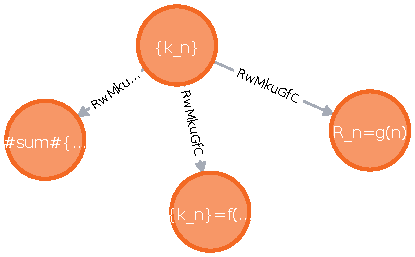
\includegraphics{求前n项和.pdf}
	\caption{求前n项和实例化图谱}
	\label{求前n项和}
\end{figure}

在neo4j图数据库中添加完实例化定理后,继续对题目的文本信息进行输入,题目的
已知事实和求解目标再网页端的输入如图5-5(a)所示。题目输入完成后,会在网页首先
显示自然语言理解的结果,是以json的数据格式存储三元组信息,具体json数据如图
5-5(b)所示。题目的json解析的结果是由三部分组成的,第一部分是自然语言命名体
识别的结果,它最终是以一个”entities“数组的形式记录解析结果,构成json数据的
第一部分;第二部分是关系抽取的结果,即抽取题目中涉及的所有实体之间的关系,最终
生成了三元组数组,其中三元组是有所分类的,题干三元组”SteamRelation“以及小问
三元组“substeamRelation”,在形式上可以通过三元组中的“asking”字段进行区分,
题干三元组的“asking"均为0,而小问三元组中的“asking”是”1-8“之间的一个数字;
第三部分是一些附加信息,为了前后端通信所添加的字段,”questionId“
表示题目的唯一标识,”fakeText“表示题目的文本描述,在后续的类人解答中可以应用。
整个题目的知识图谱如图5-5(c)所示。
\begin{figure}[htbp]
	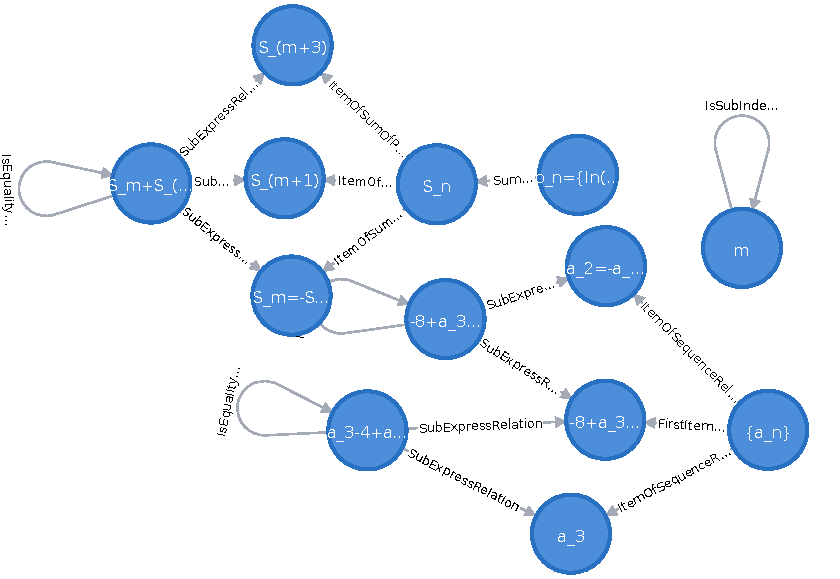
\includegraphics{题目图谱.pdf}
	\caption{题目知识图谱}
	\label{题目图谱}
\end{figure}
********************
********************

题目实例子图生成之后,将进入后端的推理模块,推理引擎会去neo4j
图数据库中读取题目子图,读取的方式是根据题目提供的唯一标签,即
”questionId"这个字段去获取子图。由前文4.3.1节中所介绍推理引擎
的逻辑架构可知,第一层逻辑层就是解构题目子图和实例化子图,并完成
内存中推理的各类数据结构的初始化工作。“QuestionTripls”是保存
题目图谱中的所有已知条件三元组,包括求解目标的三元组,设置成全局
变量,具体的三元组信息如表5-3所示。

推理引擎的第二层逻辑结构是匹配模块,在匹配之前会对初始化的三元组
集合进行重排,重排的依据是依据关系中的字段“Order”进行排序,主要
目的是为了确保相同三元组有个相对的序,这个序来源于原始的题目描述,
通过“Order”字段记录描述的先后顺序。对题目三元组集合和实例化三元组
集重排后封装成map的数据结构,其中key为三元组中的关系,value值为
包含该关系的所有三元组并且有序,因此最终选择的是优先队列进行存储
有序三元组。如表5-4和5-5所示。分别为题目和实例化定理的匹配数据结构。
若实例化定理匹配成功,引擎会生成一张实例化定理中形式参数映射至
题目中具体参数的置换表,为了保留更多的信息,置换表的key和value值
均为实体类型的数据,每一个匹配成功的实例化定理都有一张置换表,
实例化置换表对于后续的推理至关重要。如表5-6是“3”实例化的置换表。
*******************
*****************
****************

匹配成功后,会进入知识的产生和更新模块。其中知识的产生包括包含两个
部分,首先需要进行参数置换,即对实例化中参数转换成具体的题目中参数
,置换完参数后需要调用计算平台服务,计算后的结果会进一步封装成三元组
,最终新知识同样是以推理最小单位三元组的形式存储。新知识产生的关键
一步在于参数置换,而参数置换就是依赖于匹配逻辑中的置换表。因此置换表
是整个推理引擎中的重要数据结构,在引擎中各个逻辑层都有所应用。新知识
产生后在内存中以三元组的形式存储,同样需要将新知识插入到原始的题目
知识图谱中,实例化“3”具体的插入方式如下:首先解析得到实例化的结论
三元组部分,如图5-8所示,结论三元组的头实体在置换表中可以找到对应
的映射实体,属于旧知识无需新生成实体,尾实体是计算服务得到的新知识,
在图谱中生成新的实体,实体名为“”,实体类型与实例化的尾实体类型相同。
关系“”是原有知识图谱中缺失关系,需要在头实体和新生成的尾实体之间插入。
**************
由上述讲解,参数置换和知识更新均依赖于置换表结构,对于每一个实例化
定理都有不同的置换表和更新策略。本题匹配成功的实例化知识更新情况如
表5-7所示。图匹配完成知识更新和正确停机,求解成功之后的图谱如图5-6所示。
\begin{figure}[htbp]
	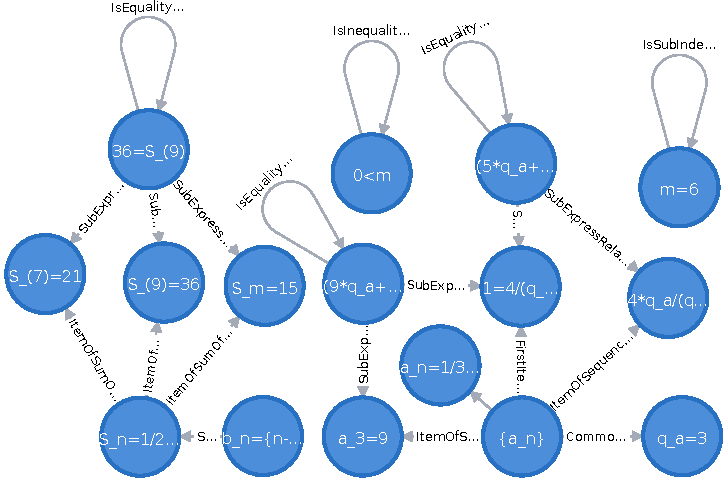
\includegraphics{求解结果图.pdf}
	\caption{题目更新知识图谱}
	\label{求解结果图}
\end{figure}
\subsection{批量测试}

\section{后续工作展望}


\end{document}